\documentclass{beamer}
%\documentclass{easytikz}


\usepackage{default}
\usepackage{tikz}

\usepackage[utf8]{inputenc}
\usepackage[T1]{fontenc}

\usetikzlibrary{shapes.geometric, arrows}
\usetikzlibrary{positioning}

\tikzset{
  se/.style={rectangle, rounded corners, minimum width=3cm, minimum height=1cm,text centered, draw=black, fill=red!30},
  io/.style={trapezium, trapezium left angle=70, trapezium right angle=110, minimum width=3cm, minimum height=1cm, text centered, draw=black, fill=blue!30},
  op/.style={rectangle, minimum width=3cm, minimum height=1cm, text centered, draw=black, fill=orange!30},
  cn/.style={diamond, minimum width=3cm, minimum height=1cm, text centered, draw=black, fill=green!30},
  node distance=5mm
}

\begin{document}

\begin{frame}[fragile]

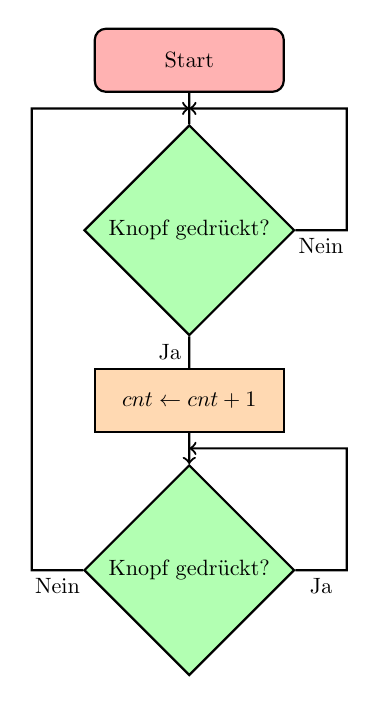
\begin{tikzpicture}[thick,scale=0.8, every node/.style={transform shape}]
\node[se] (start) {Start};
%\node[op, below=of div] (set) {$a=b,\ b=r$};
\node[cn, below=of start] (condon) {Knopf gedrückt?};
\node[op, below=of condon] (cnt) {$cnt \leftarrow cnt + 1$};
\node[cn, below=of cnt] (condoff) {Knopf gedrückt?};

%
\draw[->] (start) -- (condon) coordinate[midway] (startedge)
(condon) -- node[left] {Ja} (cnt)
(cnt) -- (condoff) coordinate[midway] (condonedge);
\draw[->] (condon) -- node[below] {Nein} ++(2.5,0) |- (startedge);
\draw[->] (condoff) -- node[below] {Ja} ++(2.5,0) |- (condonedge);
\draw[->] (condoff) -- node[below] {Nein} ++(-2.5,0) |- (startedge);
\end{tikzpicture}

\end{frame}

\end{document}
